
\resetcounters

\bibliographystyle{asp2010}

\markboth{Masters and Braatz}{A Spectral Pipeline for the Green Bank Telescope}

\title{A Spectral Pipeline for the \ssindex{observatories!Earth-based!Green Bank Telescope (GBT)}Green Bank Telescope}
\author{Joe~Masters and Jim~Braatz
\affil{NRAO Headquarters, 520 Edgemont Rd, Charlottesville, VA 22903-2475}}

\aindex{Masters, J.}
\aindex{Braatz, J.}

\begin{abstract}
Recently, historic \ssindex{observatories!Earth-based!Green Bank Telescope (GBT)}Green Bank Telescope (GBT) data was made available to the user community through the \ssindex{archives!multiple!National Radio Astronomy Observatory (NRAO) data archive}National Radio Astronomy Observatory (NRAO) data archive service.  In support of this archive, and to offer quick access to \ssindex{observatories!Earth-based!Green Bank Telescope (GBT)}GBT data, NRAO has instituted the \ssindex{observatories!Earth-based!Green Bank Telescope (GBT)}GBT \ssindex{data!pipelines!reduction}Pipeline Project to provide reduced spectra from public \ssindex{observatories!Earth-based!Green Bank Telescope (GBT)}GBT datasets to the user community.
\end{abstract}

\section{Introduction}

The GBT \ssindex{data!pipelines!reduction}Pipeline Project has two goals. The first is to produce an automated data processing \ssindex{data!pipelines!reduction}pipeline that can generate quick-look spectra for about 80\% of all spectral line data observed with the \ssindex{observatories!Earth-based!Green Bank Telescope (GBT)}GBT, including data observed with the VEGAS spectrometer \citep{2012arXiv1202.0938A} in standard observing modes. For certain types of science data, this project will produce archive-ready data products, including a ``summary sheet" for each reduced spectrum with accompanying header and \ssindex{statistical analysis}statistical information. A second goal of the \ssindex{data!pipelines!reduction}Pipeline Project is to prepare tools that assist with certain potentially labor-intensive data processing tasks, such as calibrating and mapping K-band Focal Plane Array observations \citep[see][]{2011ASPC..442..127M}.

Through various approved observing programs, the \ssindex{observatories!Earth-based!Green Bank Telescope (GBT)}GBT has taken pointed observations to measure HI profiles toward several thousand galaxies. Here we show early results of the quick-look \ssindex{data!pipelines!reduction}pipeline for \ssindex{astronomy!extragalactic}extragalactic HI observations. The \ssindex{observatories!Earth-based!Green Bank Telescope (GBT)}GBT \ssindex{data!pipelines!reduction}Pipeline project plans to provide HI spectra of galaxies to the NRAO data archive and to the \ssindex{databases!individual!NED (NASA Extragalactic Database)}NASA Extragalactic Database this year.

\section{\ssindex{radio frequency interference (RFI)}RFI Excision}

Most \ssindex{astronomy!extragalactic}extragalactic HI spectra are affected by \ssindex{radio frequency interference (RFI)}RFI at some level.  The ``before and after" plots in Figure~\ref{fig:RFIfigure} demonstrate the effectiveness of our initial \ssindex{radio frequency interference (RFI)}RFI flagging approach for particularly heavy \ssindex{radio frequency interference (RFI)}RFI.  We have been developing the quick-look \ssindex{data!pipelines!reduction}pipeline for only a few weeks, so the automated \ssindex{radio frequency interference (RFI)}RFI excision we apply is rudimentary, but already effective. We examine each integration for broadband \ssindex{radio frequency interference (RFI)}RFI (excessive spectral baseline ripples) and flag integrations based on the total power in low-order \ssindex{methods!Fourier}Fourier components. We then calibrate and average the data. Finally we flag narrow-band \ssindex{radio frequency interference (RFI)}RFI using an iterative, median filter approach.

\begin{figure}[ht!]
\centering%
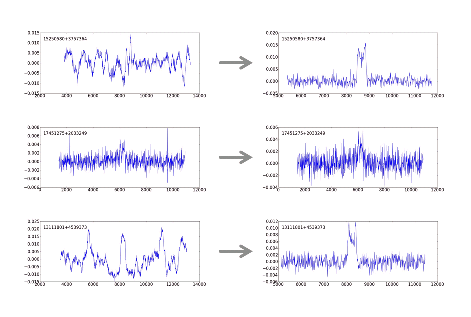
\includegraphics[width=5in]{part7/Masters_P66/P66_f1}
\caption{\ssindex{radio frequency interference (RFI)}RFI excision of three example spectra.  Plots on the left are before \ssindex{radio frequency interference (RFI)}RFI excision and plots on the right are the removal of bad component spectra and/or bad channels.}
\label{fig:RFIfigure}
\end{figure}

\subsection{Baseline Subtraction}

Like \ssindex{radio frequency interference (RFI)}RFI excision, the best methods for baseline subtraction will take some experimentation.  However, baseline subtraction in the \ssindex{data!pipelines!reduction}pipeline will likely consist of:

\begin{itemize}
\item a selectable baseline fitting range (i.e. channels, velocity)
\item a tunable order of polynomial for fit
\item a choice of sinusoidal or \ssindex{methods!Fourier}Fourier fitting
\end{itemize}

\subsection{Data Grouping and Selection}

The \ssindex{data!pipelines!reduction}pipeline will allow users to select which data to process.  In some cases, this will be a filtered set of data.  In other cases, it will simply be a way of grouping data together during processing without any reduction in the total amount of data being processed.  For example, the user may process every scan pair or all scans for a target in an observation.  Furthermore, a user may choose either to separate or combine \ssindex{astronomy!polarization}polarizations in their processing.  Other processing filters may include the source name, the spectral window or included/excluded regions of spectra (e.g. by channels or velocity).

\section{Automatic vs Manual Operation}

\paragraph{Automatic}

The first, and in some ways most sophisticated mode, is for the \ssindex{data!pipelines!reduction}pipeline to run without user input.  Ideally, the \ssindex{data!pipelines!reduction}pipeline will run automatically at the completion of an observation.  Alternatively, the user should just direct the \ssindex{data!pipelines!reduction}pipeline to a particular input file or even a Project Identifier.  In this mode, the \ssindex{data!pipelines!reduction}pipeline will use information contained within the dataset(s) to make educated guesses about what calibration techniques and parameter values are appropriate for the observation.

A user may use the automatic mode on an entire dataset or a subsection of integrations.

\paragraph{Manual}

The user will also be able to run the \ssindex{data!pipelines!reduction}pipeline with full, or close to full, control over many calibration and output settings.  This may be useful when the user believes she can make better choices about parameter values.

\section{Data Products}

By default, the \ssindex{data!pipelines!reduction}pipeline will produce the following data products.  Depending on options set by the user, the format of each of these products may vary.
\begin{enumerate}
\item Calibrated single dish \ssindex{data formats!FITS}FITS (SDFITS) with a spectrum per target per spectral window
\item A summary web page including images of spectra, header information and basic statistics/analysis
\end{enumerate}

These products are also oriented toward use by the archive.  They will be searchable by header information in the SDFITS file and in the summary page.

\subsection{Summary Information}

The \ssindex{data!pipelines!reduction}pipeline will produce a summary page (or set of summary pages) for each processing run.  The format may be PDF, HTML or plain text.

It will include:
\begin{itemize}
\item A plot of each calibrated spectrum with high-level \ssindex{data!metadata}metadata for the dataset according to the data selection parameters.  By default, this will produce a spectrum for each target.
\item Weather information
\item Basic statistics
\end{itemize}

\section{Future work}

The initial approach is to run the \ssindex{data!pipelines!reduction}pipeline on the Green Bank network.  At a later stage, the \ssindex{data!pipelines!reduction}pipeline may be controllable from a web interface or able to be run on a user's home computer.

Likewise for data product retrieval.  Initially the data produced by the \ssindex{data!pipelines!reduction}pipeline will be accessible on the Green Bank network.  Later, data products may be retrieved either from an archive access interface or another web interface.  If the \ssindex{data!pipelines!reduction}pipeline is run on a user's home computer, then the data products will be produced on that machine.

\acknowledgements We would like to thank the National Science Foundation for funding this work.

\bibliography{editor}
